\documentclass[../DefinizioneDiProdotto.tex,lanscape]{subfiles}
\begin{document}

\section{Diagrammi riassuntivi package}
	Di seguito sono riportati tutti i package dell'applicativo per chiarire la relazione tra le componenti e le classi al suo interno visto l'utilizzo del pattern MVP. Per chiarezza ed esigenza di spazio le classi rappresentate all'interno dei package sono rappresentate senza metodi e attributi.

	

	\subsection{model::dataaccess::service}
		Il package \verb|service| è incaricato di gestire i download, lo storage e la rimozione dei dati contenuti nel databese SQLite locale. Le dipendenze con tale package sono tutte risolte attraverso l'uso della dependency injection (diagramma \ref{diPackage}).

\begin{figure}[h]
	\centering
	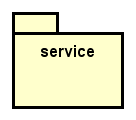
\includegraphics[scale=0.6]{img/RelationPackage/service}
	\caption{Package model::dataaccess::service}
	\label{servicePackage}
\end{figure}


\newpage
	\subsection{model::dataaccess::dao}
		Il package \verb|dao| è incaricato della costruzione dell'oggetto \verb|BuildingMap| attraverso altri componenti (\verb|-Table|) tramite i dati scaricati in formato Json o prelevati dal database SQLite locale. Il package è utilizzato solo dal package \verb|service| e le classi Factory sono utilizzate tramite la dependency injection.

\begin{figure}[h]
	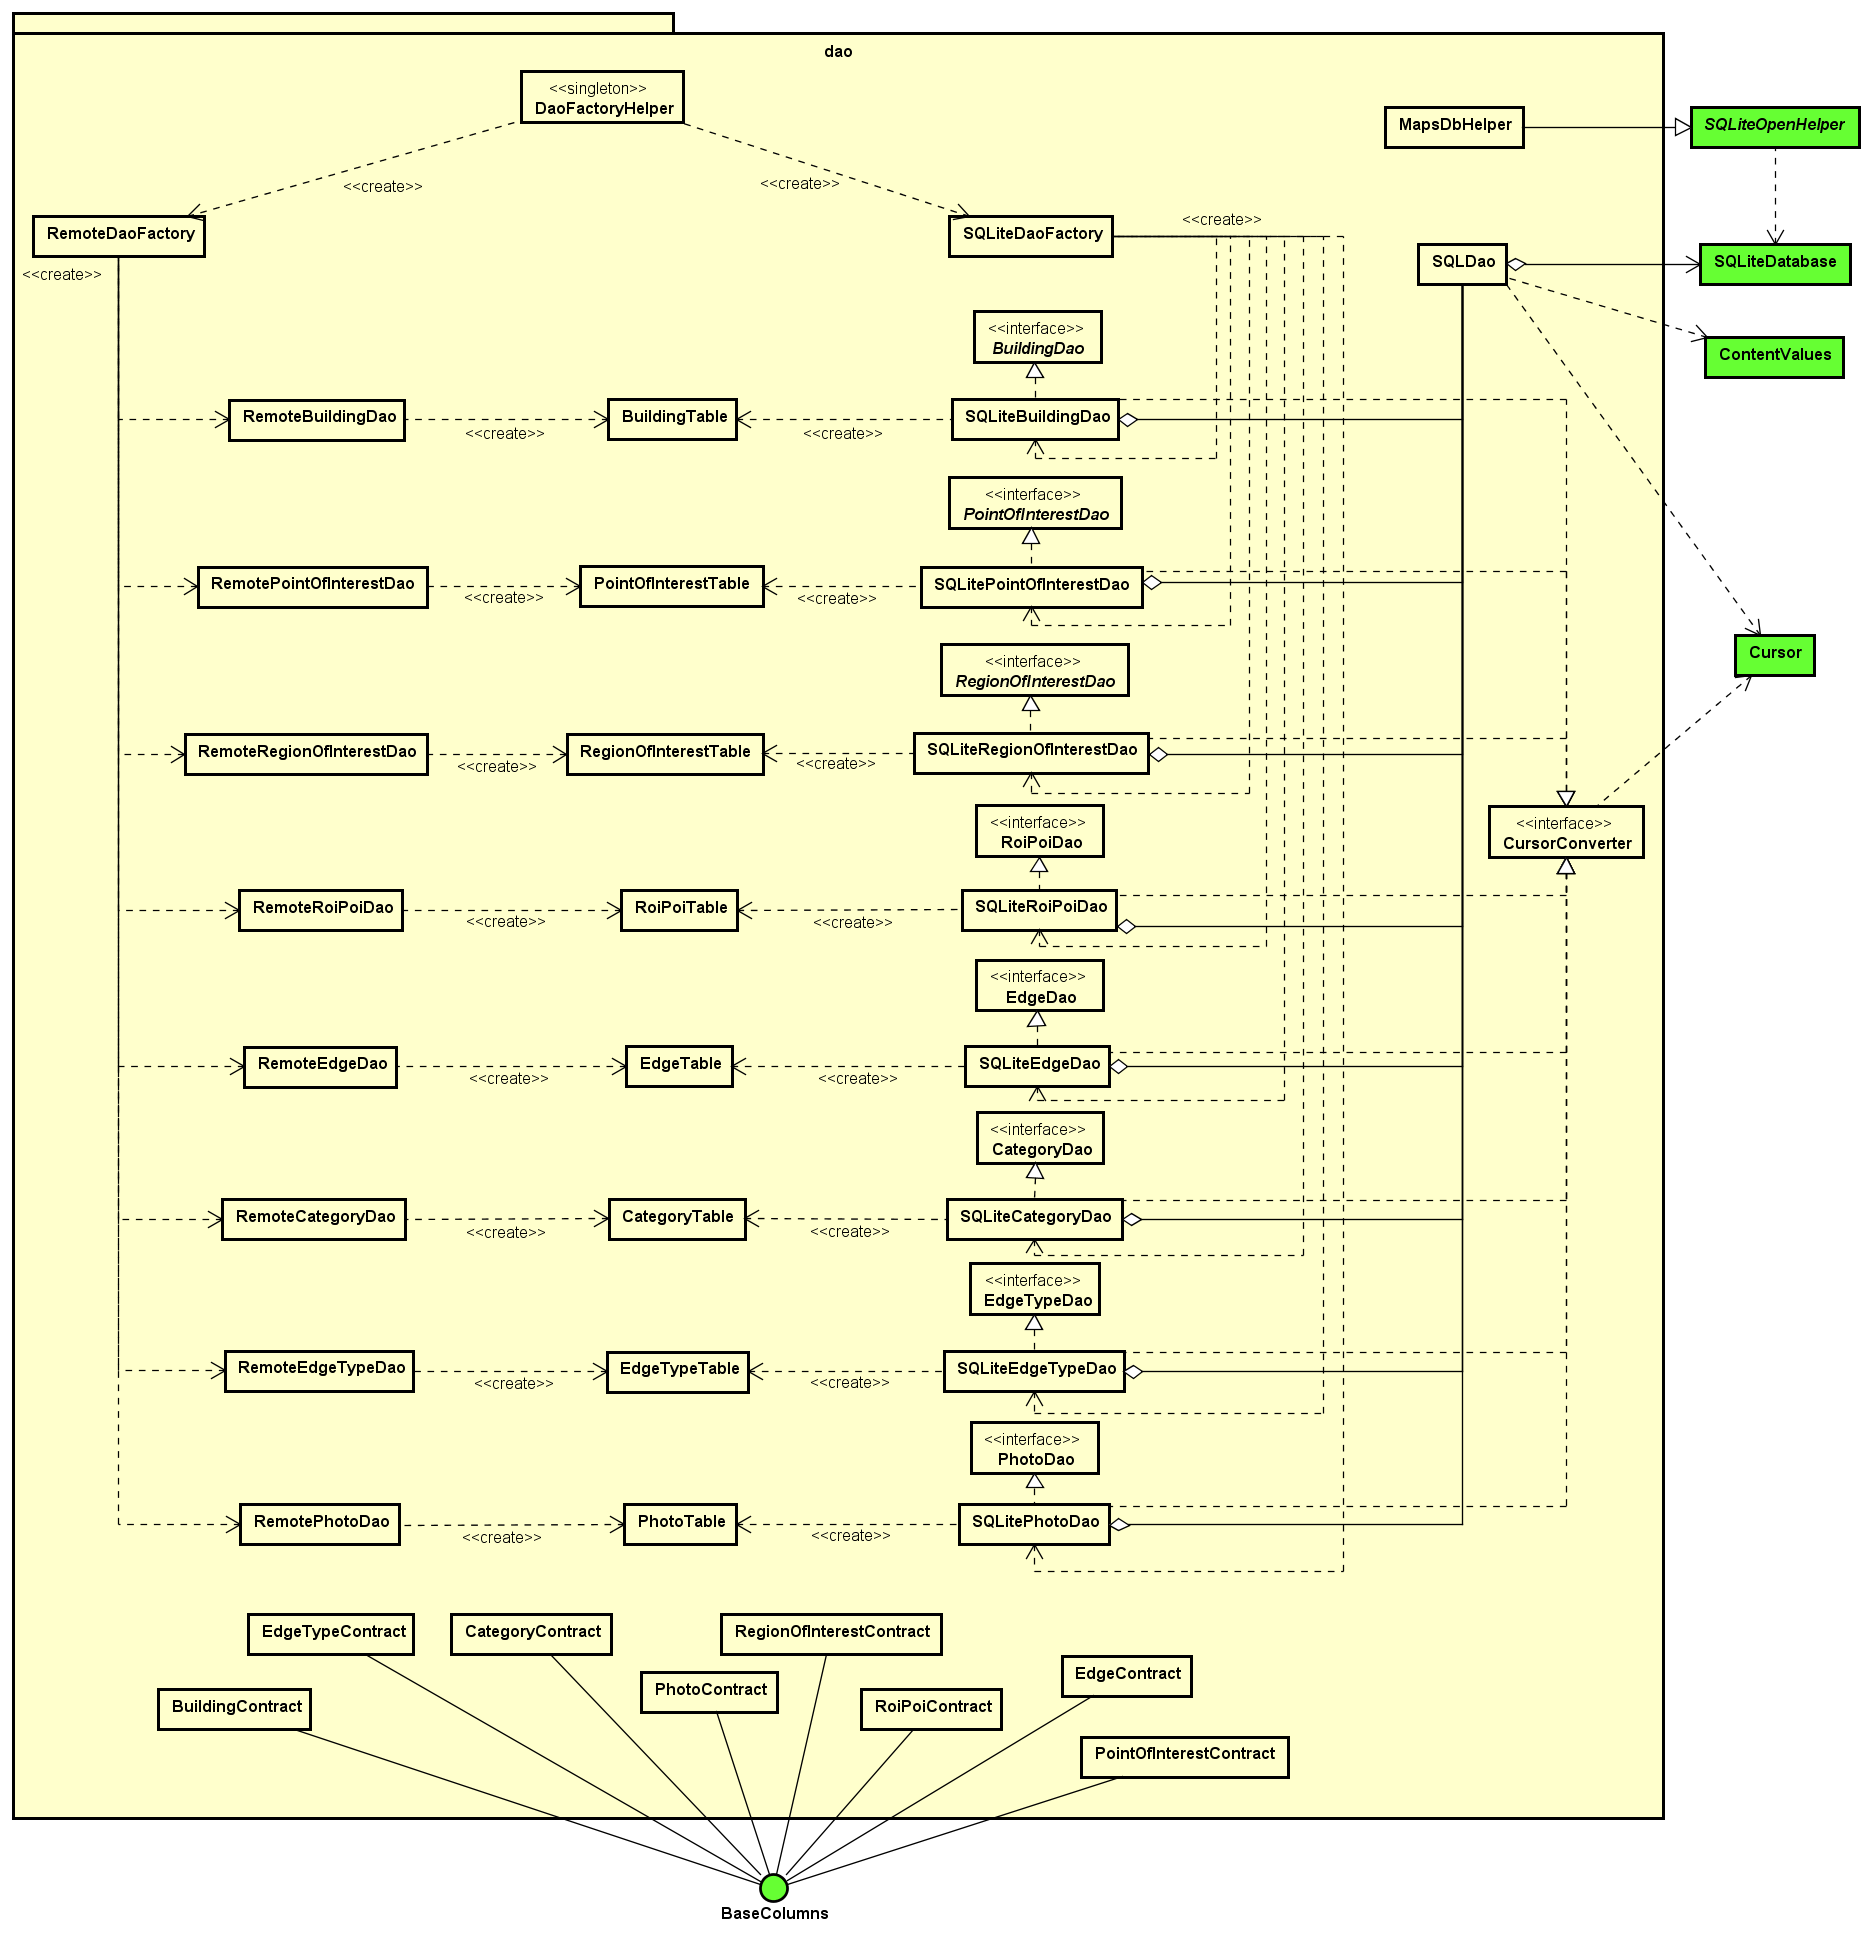
\includegraphics[width=\textwidth]{img/RelationPackage/dao}
	\caption{Package model::dataaccess::dao}
	\label{daoPackage}
\end{figure}


\newpage

	\subsection{model::navigator::graph}
		Il package \verb|graph| è incaricato di permettere la costruzione del grafo rappresentante l'edificio, l'oggetto \verb|MapGraph|. Esso è composto dai package: \verb|area|, \verb|navigationinformation|, \verb|edge| e \verb|vertex|.  Ha relazioni con il package esterno \verb|model| con la classe \verb|NavigationManagerImp| il quale contiene un campo \verb|MapGraph|.

\begin{figure}[h]
	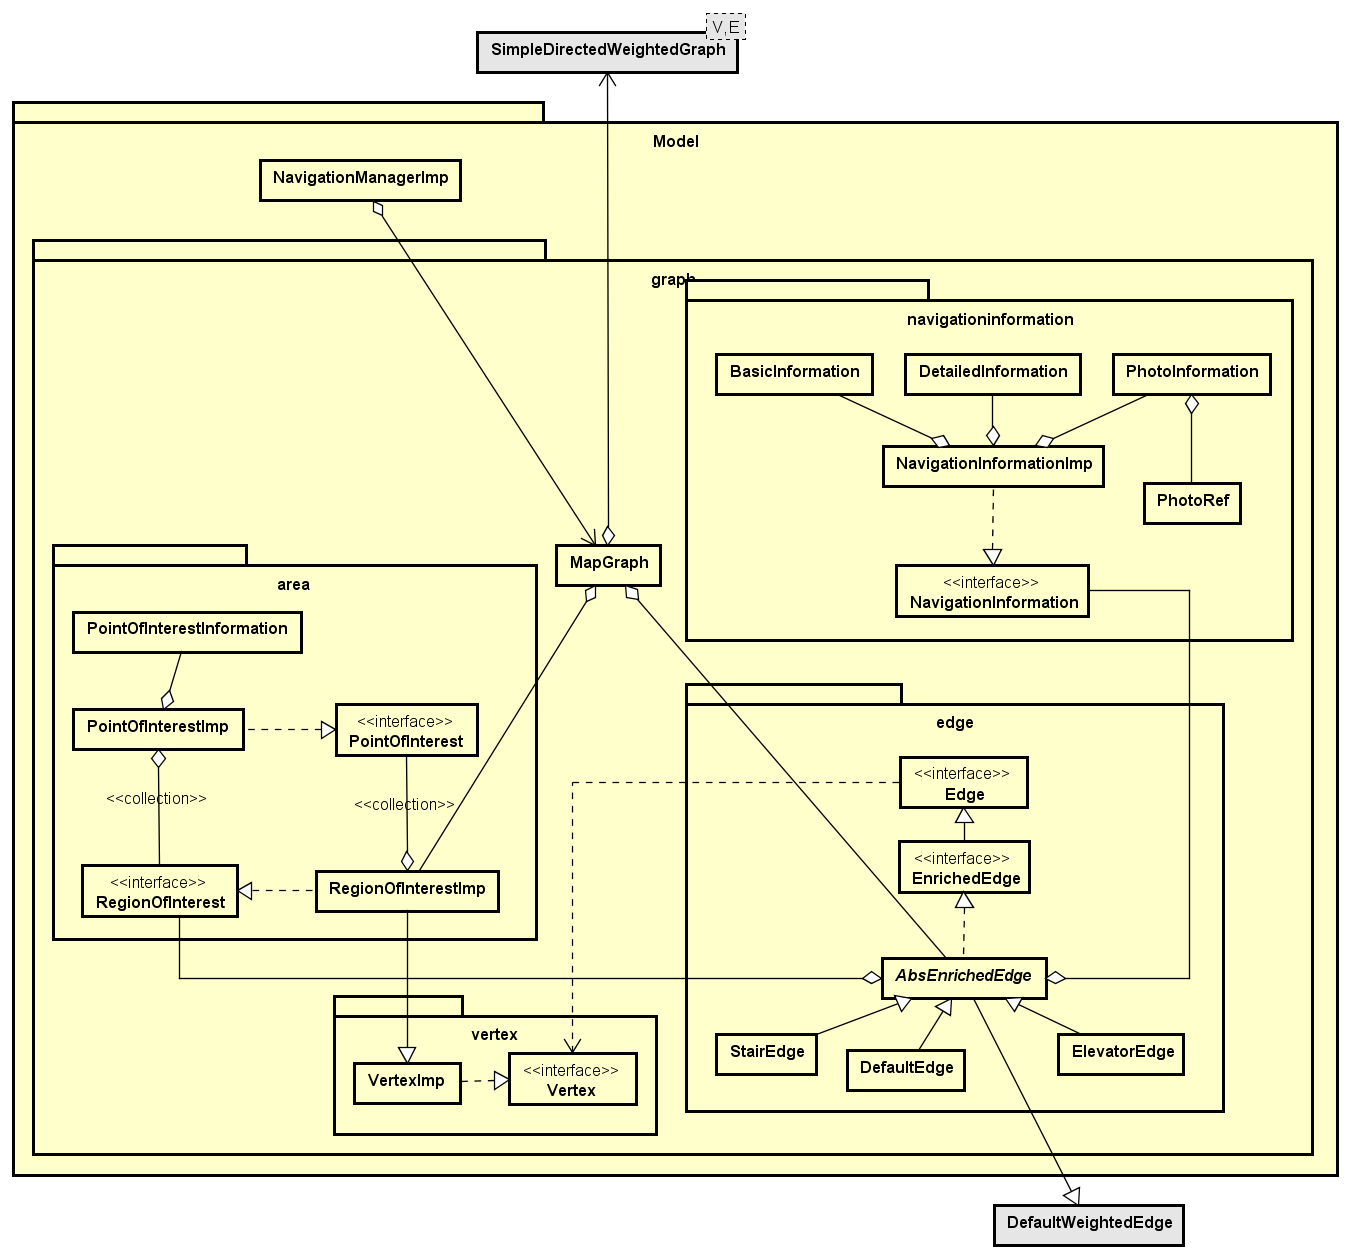
\includegraphics[width=\textwidth]{img/RelationPackage/graph}
	\caption{Package model::navigator::graph e relazioni con il package esterno model}
	\label{graphPackage}
\end{figure}


\newpage
	
	\subsection{model::navigator}
		Il package \verb|navigator| ha il compito di eseguire i calcoli e di fornire le prossime istruzioni per permettere all'utente di navigare. Contiene il package \verb|graph| e \verb|algorithm|, quest'ultimo fornisce l'algoritmo di Dijkstra sul grafo fornito dal package \verb|graph|.

\begin{figure}[h]
	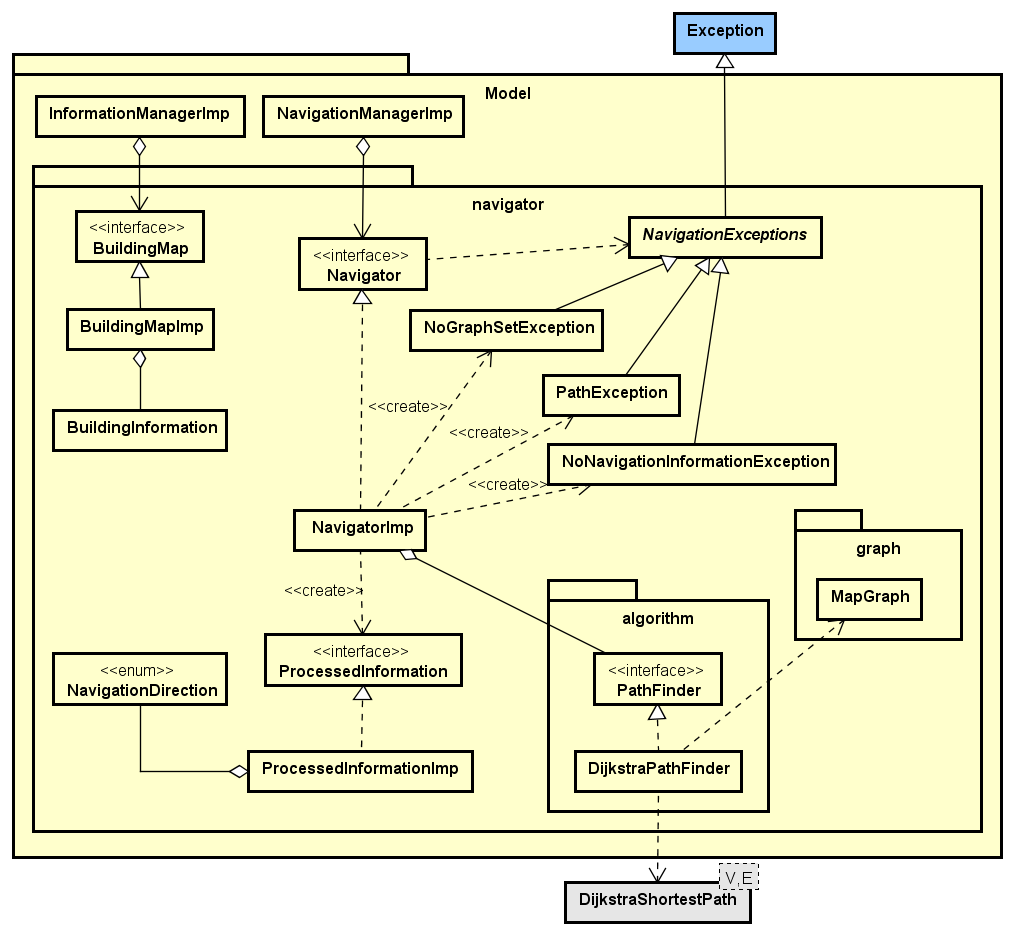
\includegraphics[width=\textwidth]{img/RelationPackage/navigator}
	\caption{Package model::navigator e relazioni con i package interni graph e algorithm e con il package esterno model}
	\label{navigatorPackage}
\end{figure}


\newpage

	\subsection{model::compass}
		Il package \verb|compass| ha il compito di calcolare l'orientamento del dispositivo fisico attraverso i dati ricavati dai sensori dello stesso. Esso attraverso l'uso di listener comunica direttamente con il \verb|presenter|.

\begin{figure}[h]
	\centering
	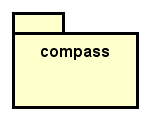
\includegraphics[scale=0.6]{img/RelationPackage/compass}
	\caption{Package model::compass e relazioni con il package presenter}
	\label{compassPackage}
\end{figure}


\newpage

	\subsection{model::usersetting}
		Il package \verb|usersetting| permette di utilizzare la funzionalità \verb|SharedPreference| offerta dall'SDK Android. Esso comunica solo con il package esterno \verb|model| che lo contiene.

\begin{figure}[h]
	\centering
	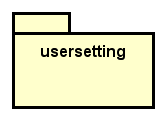
\includegraphics[scale=0.6]{img/RelationPackage/usersetting}
	\caption{Package model::usersetting e relazioni con il package esterno model}
	\label{usersettingPackage}
\end{figure}


\newpage
	\subsection{model::beacon}
		Il package \verb|beacon| permette l'utilizzo della libreria AltBeacon per interfacciarsi con la tecnologia beacon. Il package comunica con il package esterno, il \verb|model|, attraverso l'uso degli \verb|Intent| offerti dall'SDK Android attraverso i quali vengono passati oggetti \verb|MyBeaconImp|.

\begin{figure}[h]
	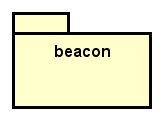
\includegraphics[width=\textwidth]{img/RelationPackage/beacon}
	\caption{Package model::beacon e relazioni con package model e librerie esterne}
	\label{beaconPackage}
\end{figure}


\newpage
	\subsection{model}
		Il package \verb|model| contiene tutta la business logic dell'applicazione che è gestita attraverso le due classi principali \verb|InformationManager| e \verb|NavigationManager|. Esse sono incaricate della gestione di tutte le sottocomponenti e della comunicazione con il \verb|presenter|.

\begin{figure}[h]
	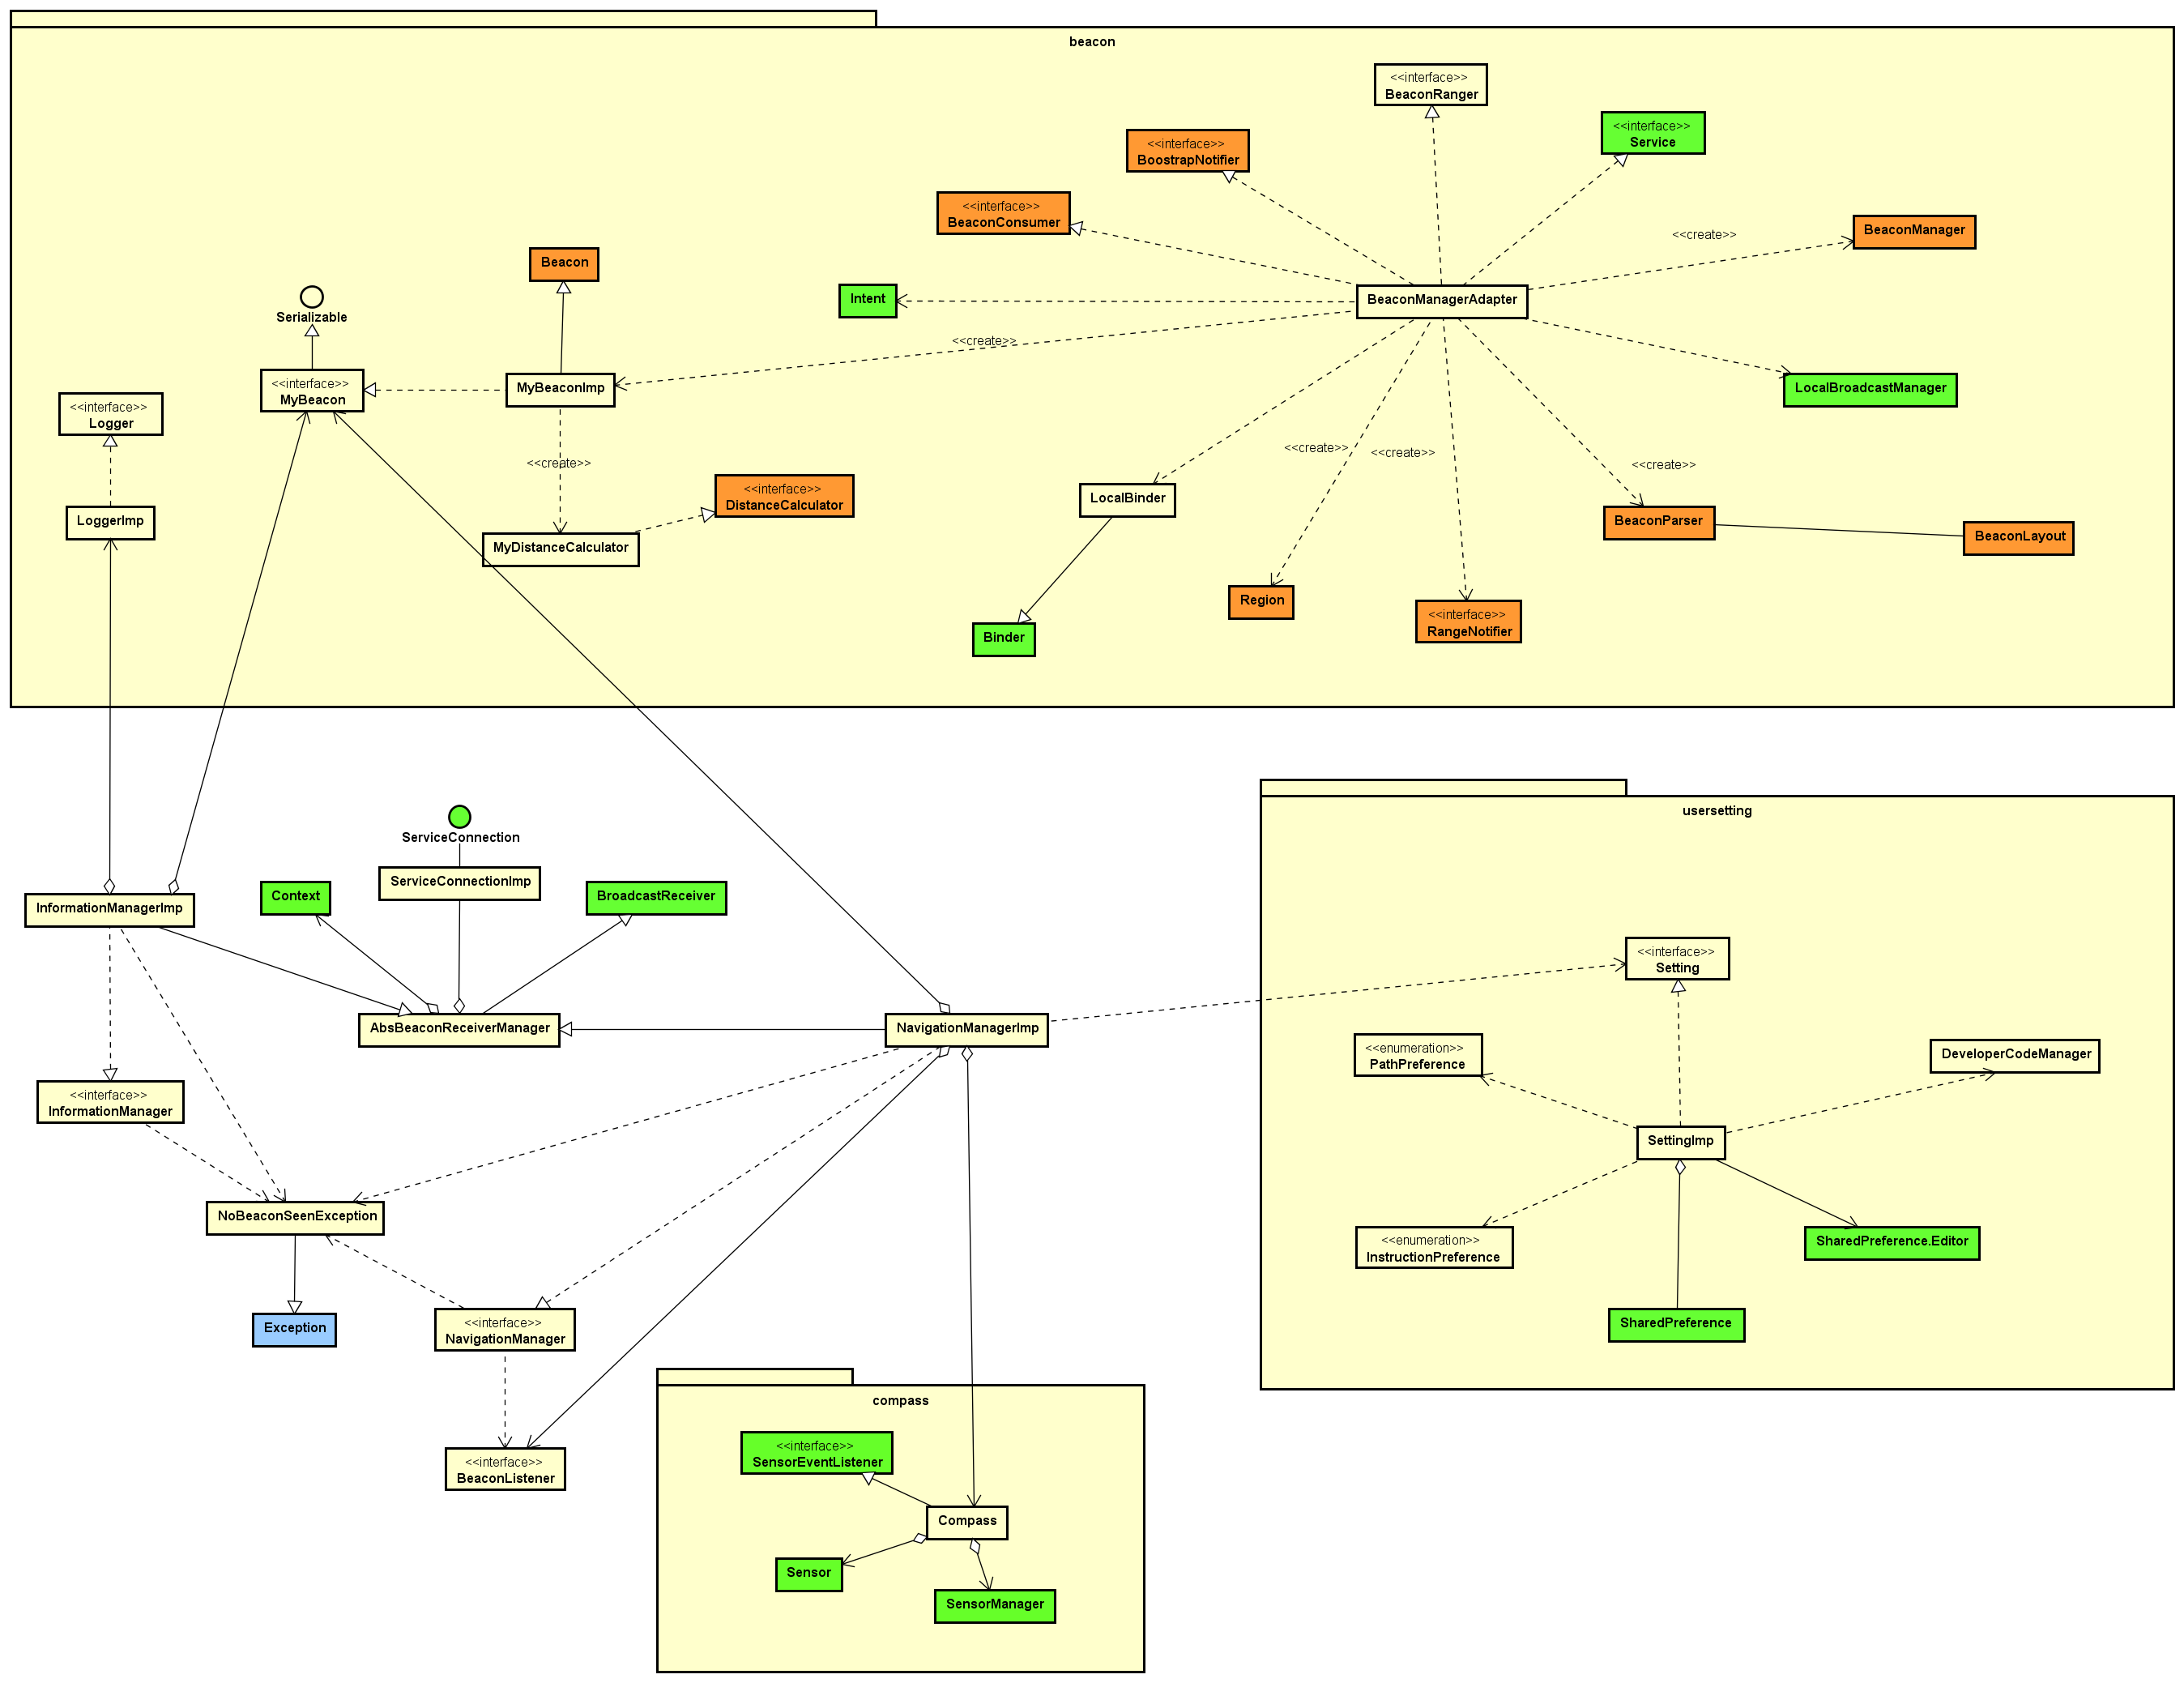
\includegraphics[width=\textwidth]{img/RelationPackage/model}
	\caption{Package model e relazioni con i package interni}
	\label{modelPackage}
\end{figure}

\newpage
	\subsection{presenter}
		Il package \verb|presenter| contiene tutte le componenti intermedie per la comunicazione tra package \verb|model| e \verb|view|. Nel diagramma \ref{presenterPackage} si mostrano le relazioni interne al package mentre nel diagramma \ref{presenter-model} si mostrano le relazioni tra le classi tra \verb|model| e \verb|presenter|.
		
		Per mantenere la leggibilità sono state rimosse relazioni con alcune componenti di Android SDK, leggendo il diagramma si tenga conto che:
		\begin{itemize}
			\item Tutte le classi con il suffisso Adapter estendono la classe esterna \verb|BaseAdapter|;
			\item Tutte le classi con il suffisso Activity estendono la classe esterna \verb|Activity| (anche MainDeveloperPresenter la estende);
			\item Tutte le classi con il suffisso Fragment estendono la classe esterna \verb|Fragment|;
			\item Ogni relazione tra le classi all'interno del package \verb|presenter| e il package \verb|model| (diagramma \ref{presenter-model}) sono risolte con la dependency injection (diagramma \ref{diPackage});
			\item Non sono mostrate le relazioni con le classi esterne \verb|Context| e \verb|Intent| perché coinvolgono pressoché tutte le classi.
		\end{itemize}
	
\begin{figure}[p]
	\centering
	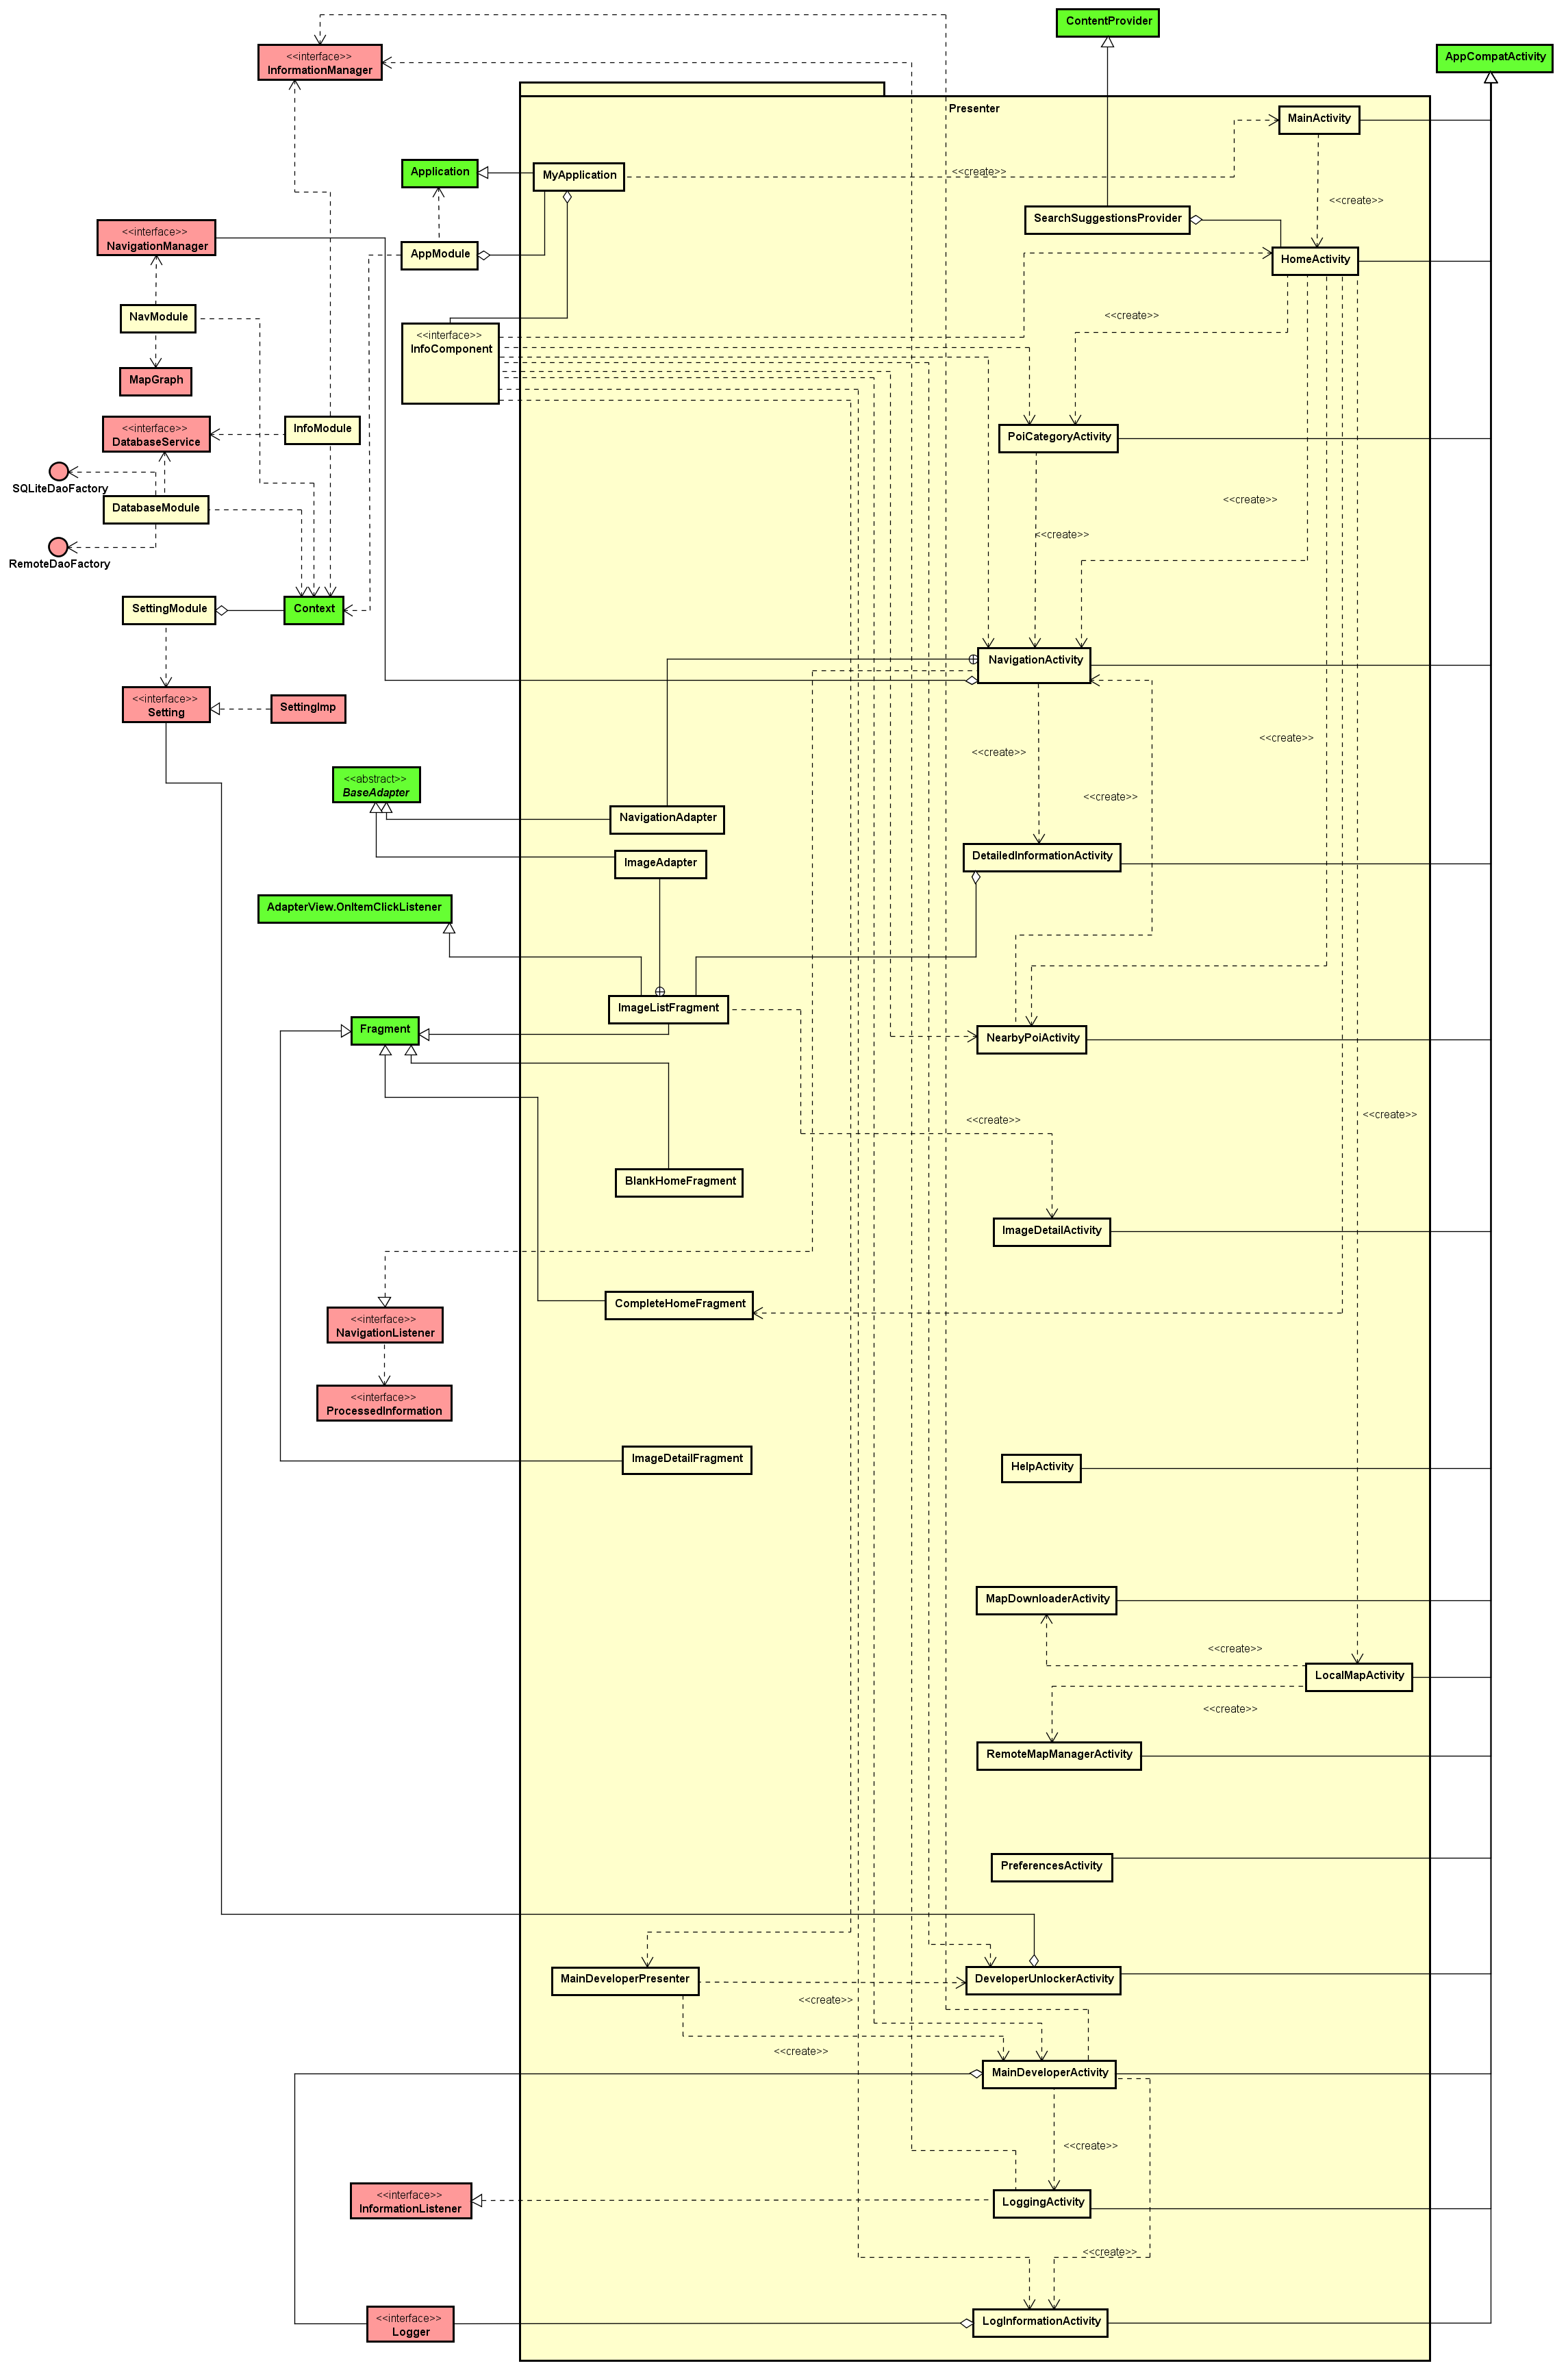
\includegraphics[height=0.9\textheight, width=\textwidth, keepaspectratio]{img/RelationPackage/presenter}
	\caption{Package presenter}
	\label{presenterPackage}
\end{figure}

\begin{figure}[p]
	\centering
	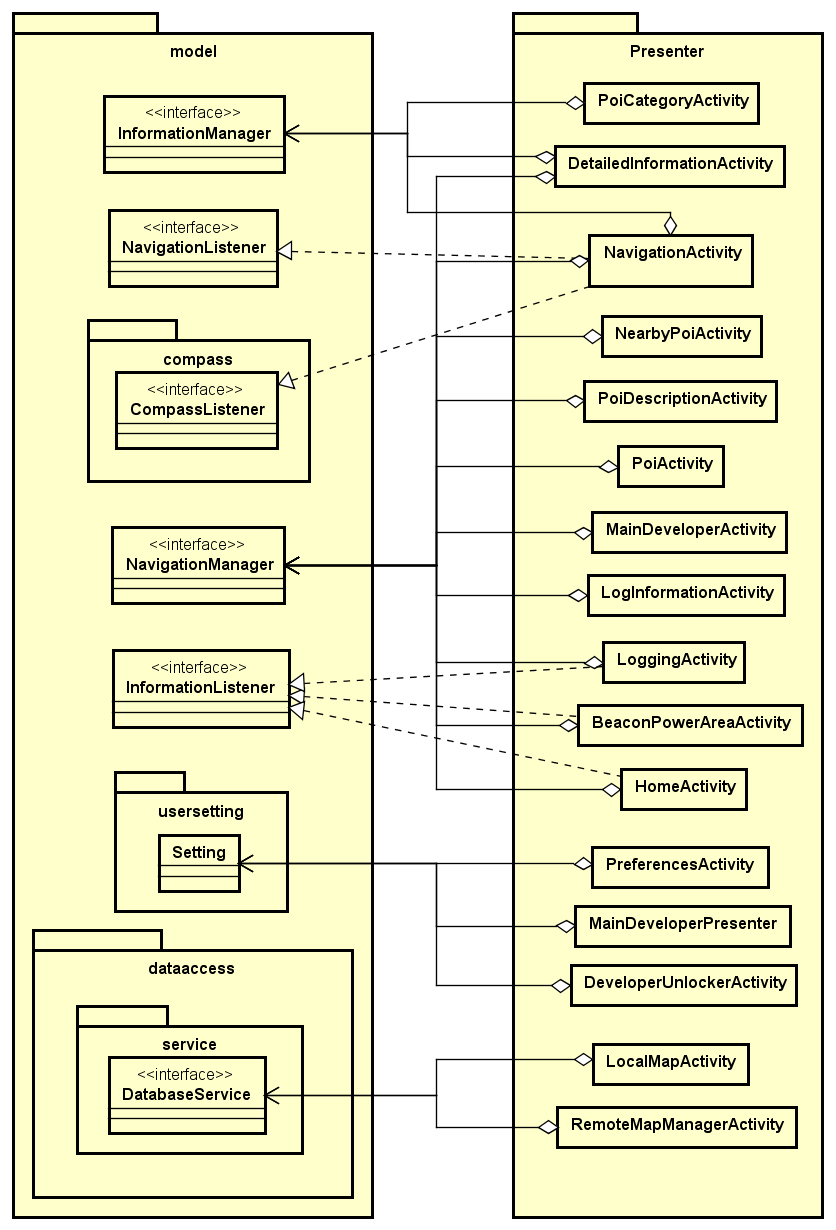
\includegraphics[width=\textwidth, keepaspectratio]{img/RelationPackage/presenter-model}
	\caption{Relazioni tra il package model e il package presenter}
	\label{presenter-model}
\end{figure}


\newpage
	\subsection{view}
		Il package \verb|view| è incaricato di contenere tutte le componenti coinvolte nella realizzazioni di elementi visualizzabili con cui l'utente potrà interagire. Per chiarezza il diagramma è stato diviso in due figure \ref{viewPackage1} e \ref{viewPackage2}. Inoltre non sono state presentate relazioni con componenti esterne offerte da Android SDK per mantenere la leggibilità del diagramma.

\begin{figure}[p]
	\centering
	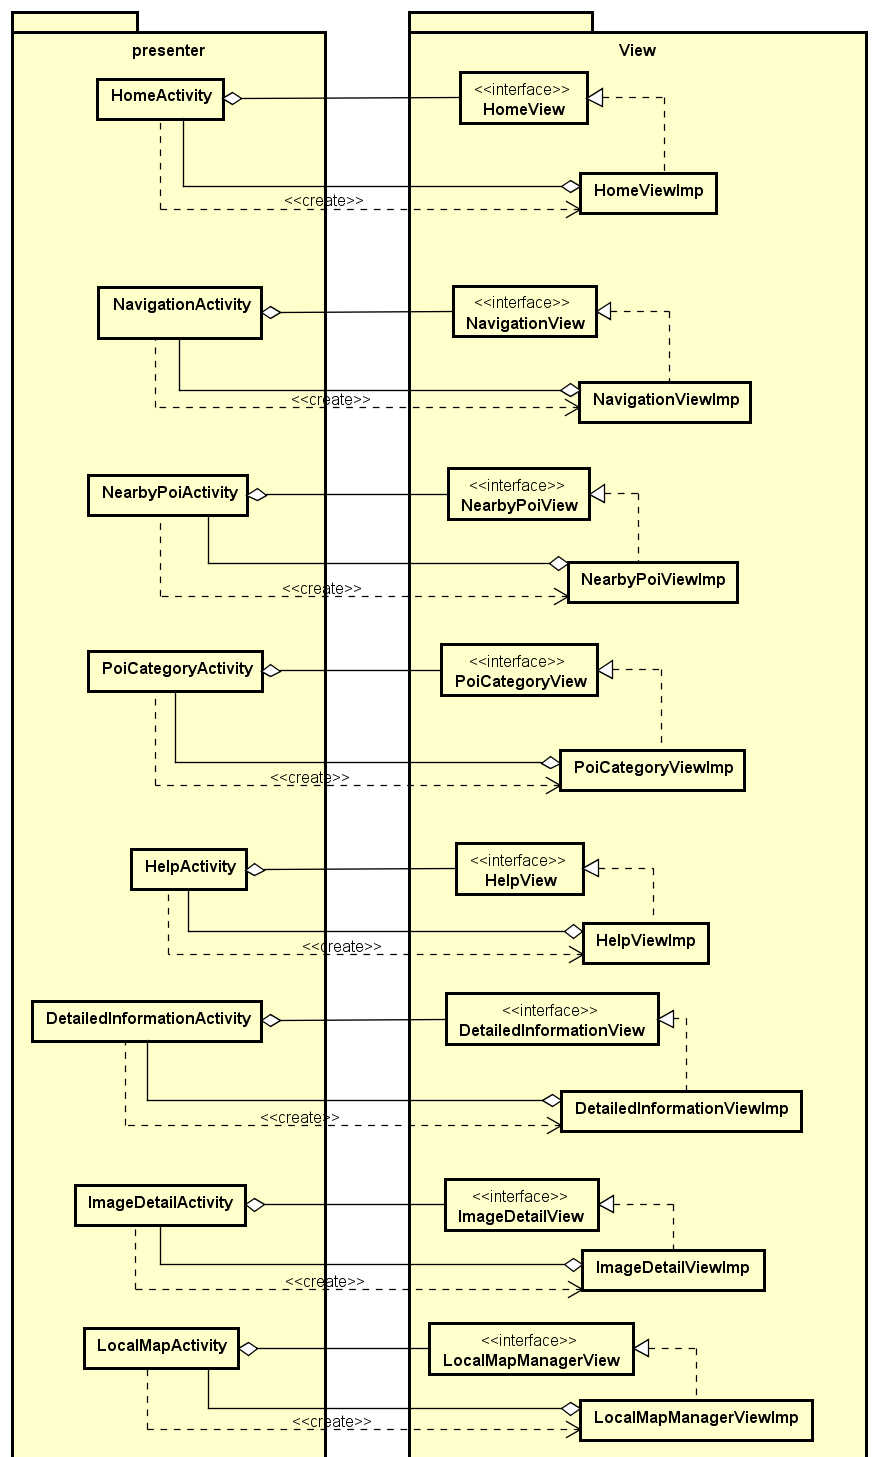
\includegraphics[scale=0.4, keepaspectratio]{img/RelationPackage/view1}
	\caption{Package view e relazioni con le componenti del package presenter (parte 1)}
	\label{viewPackage1}
\end{figure}

\begin{figure}[p]
	\centering
	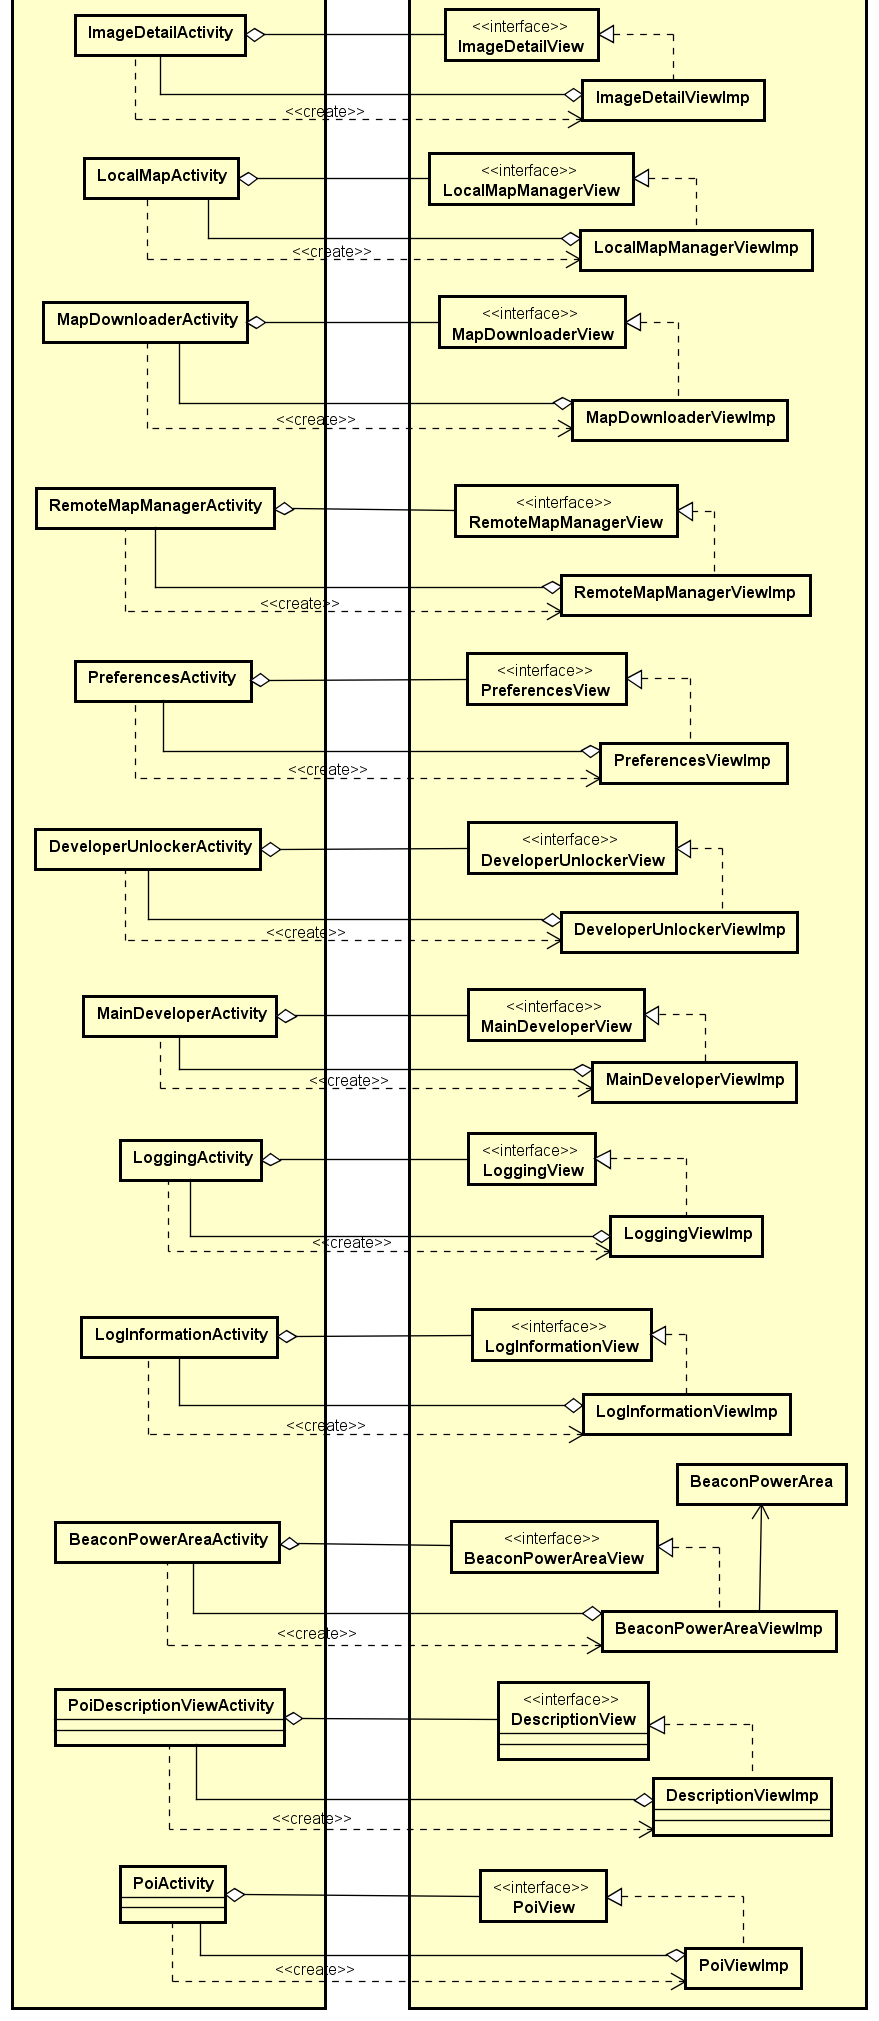
\includegraphics[height=0.9\textheight, width=\textwidth, keepaspectratio]{img/RelationPackage/view2}
	\caption{Package view e relazioni con le componenti del package presenter (parte 2)}
	\label{viewPackage2}
\end{figure}


\newpage
	\subsection{di (dependency injection)}
		Nella figura della pagina seguente si mostra come siano integrate le componenti di Dagger per implementare la dependency injection. Sempre nella figura si mostrano le relazioni tra le classi coinvolte dei package \verb|model| e \verb|presenter| rispetto al package \verb|di| il quale attraverso le classi con suffisso Module e l'utilizzo della classe amministratrice \verb|InfoComponent| permettono l'iniezione dei riferimenti delle classi del package \verb|model| nelle classi del package \verb|presenter|.
	
	
\begin{figure}[p]
	\centering
	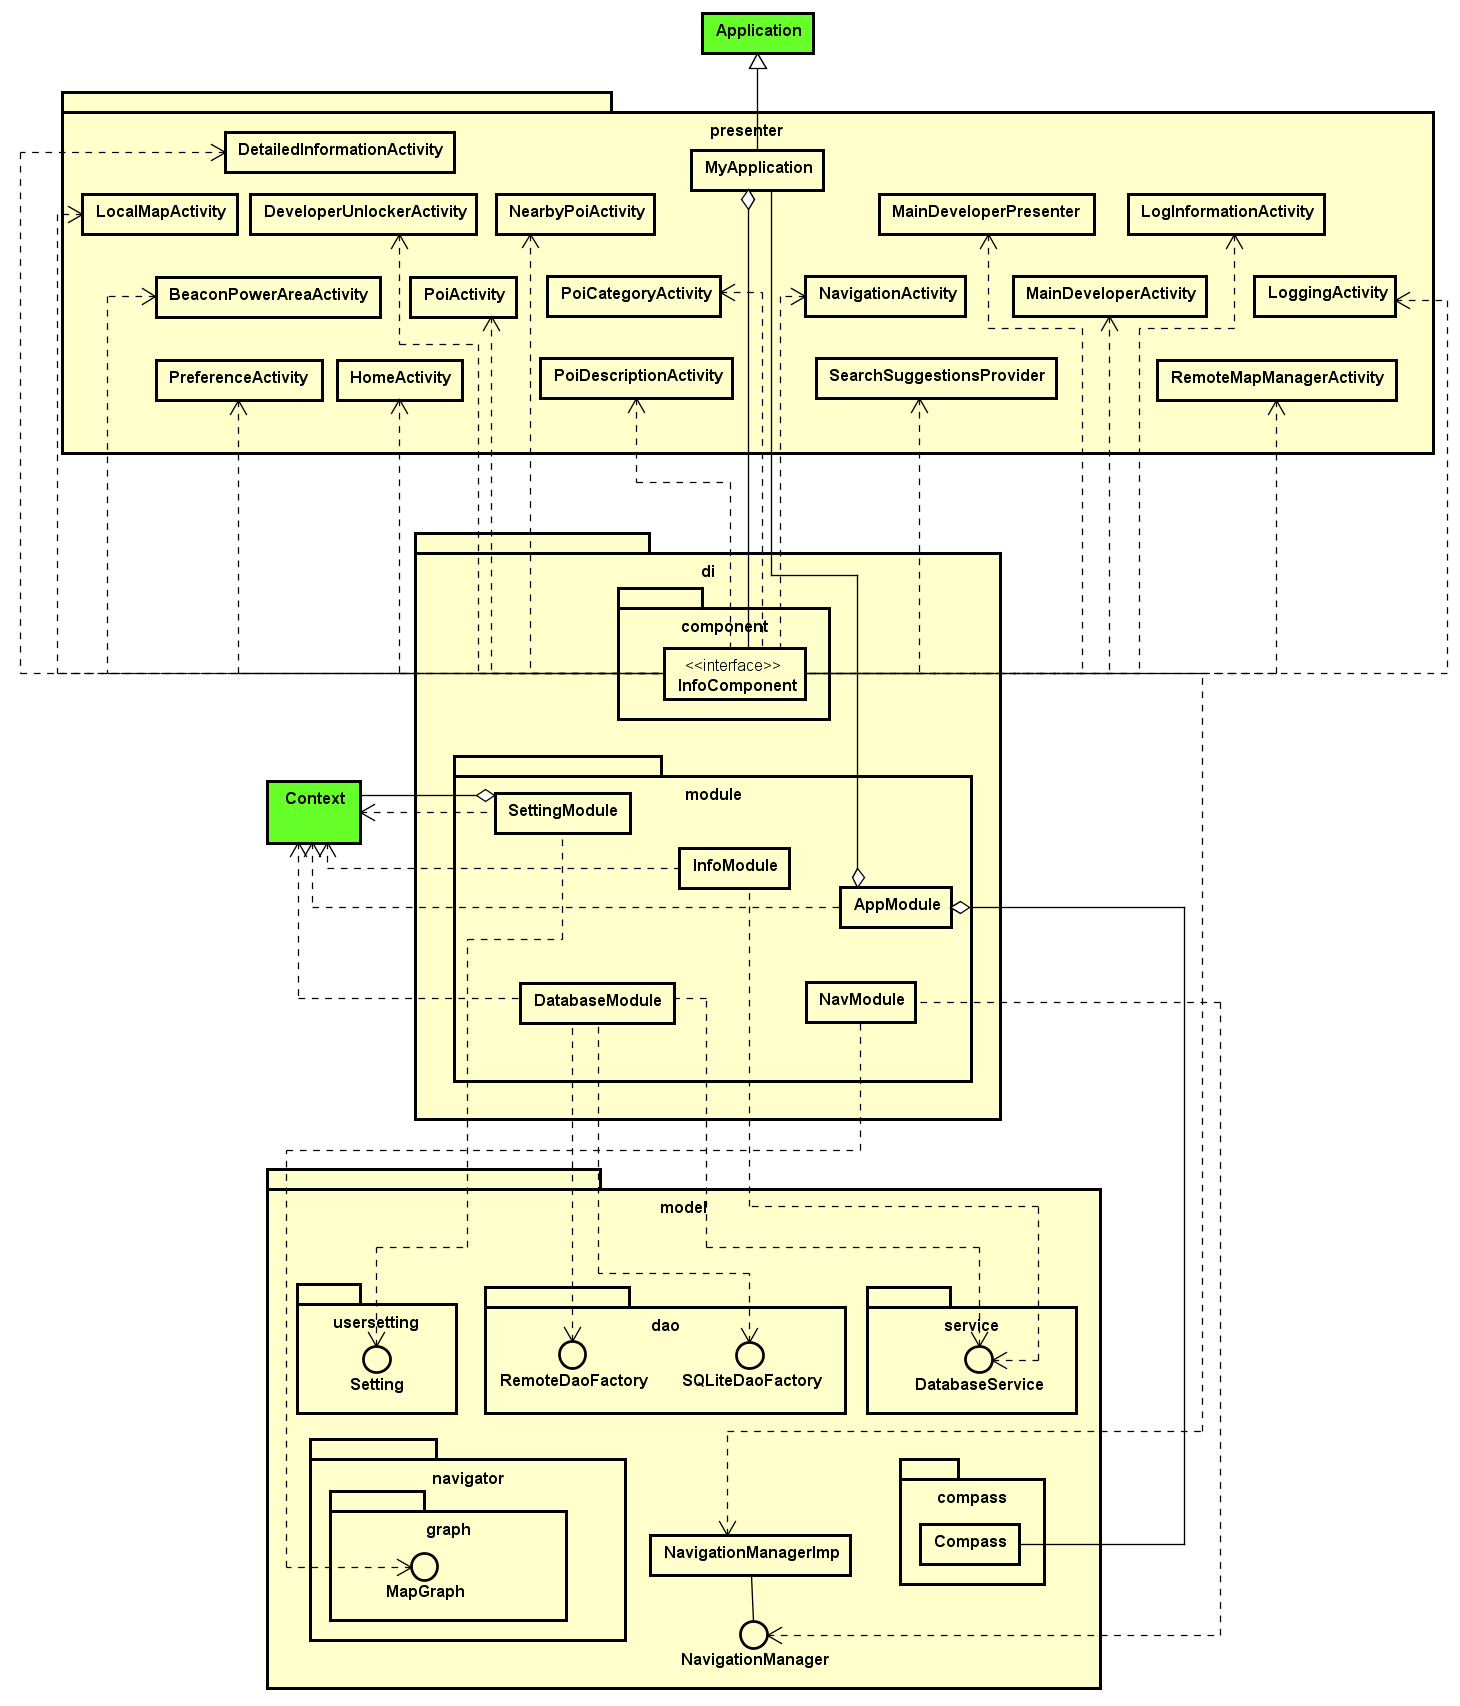
\includegraphics[height=19cm,width=\textwidth]{img/RelationPackage/di}
	\caption{Package di e relazioni con presenter e model}
	\label{diPackage}
\end{figure}

\end{document}